% HELPER FOR REPEATS:
\newcommand{\tup}[2]{\langle#1, #2\rangle}

% OUR LABEL FOR THE ``POS'' VARIABLE
\newcommand{\pos}[0]{\mbox{\it pos}}

% MY TAB STOP FOR THE PSEUDOCODE
\newcommand{\tab}[0]{\mbox{~~~~}}

%%%%%%%%%%%%%%%%%%%%%%%%%%%%%%%%%%%%%%%%%%%%%%%%%%%%%%%%%%%%%%%%%%%%%%%%%%

\section{Program Representation}

Our transformation requires a specific representation for compressed
data, as well as for programs that transform the data.  The data must
be compressed with LZ77, while the transformation must be expressed in
the cyclo-static dataflow model (e.g., in the StreamIt language).

\subsection{LZ77 Compression}

LZ77 is a lossless, dictionary-based compression algorithm that is
asymptotically optimal~\cite{wyner94optimal}.  LZ77 forms the basis
for many popular compression formats, including ZIP, GZIP and PNG, and
also serves as a generalization of simpler encodings such as Apple
Animation, Microsoft RLE, and Targa.

The basic idea behind LZ77 is to utilize a sliding window of recently
encoded values as the dictionary for the compression algorithm.  In
the compressed data stream, there are two types of tokens: {\it
  values} and {\it repeats}.  A value indicates a token that should be
copied directly to the output of the decoded stream.  A repeat
$\langle d, c \rangle$ contains two parts: a distance $d$ and a count
$c$.  It indicates that the decoder should start at offset $d$ from
the end of the decoded stream and copy a sequence of $c$ values to the
output.
%The distances are bounded, which enables the decoder to operate with a
%fixed buffer size.  
It is important to note that the count may exceed the distance, in
which case some of the values produced by a repeat operation are also
copied by that operation.  For example, a value A followed by a repeat
$\tup{1}{3}$ results in an output of ``A A A''.  An additional example
is given in Figure~\ref{fig:lz77}.

\begin{figure}[t]
\begin{minipage}{0.21in}
\mbox{~}
\end{minipage}
\psfig{figure=lz77-figure.eps,width=2.6in}
\caption{Example of LZ77 decompression.
\protect\label{fig:lz77}}
\end{figure}

\subsection{Cyclo-Static Dataflow}

The basic idea behind cyclo-static
dataflow~\cite{bilsen95-cyclostatic,LM87-i} is to represent a program
as a block diagram, in which independent components (called {\it
  actors}) communicate over FIFO data channels (see
Figure~\ref{fig:streamit}).  One can think of an actor as a function
(called repeatedly by the runtime system) that consumes items from the
input tapes and produces items on the output tapes.  Actors must
declare how many items they will produce and consume on each
execution; these I/O rates must either be constant across all
executions, or must follow a fixed cycle.  In this paper, actors may
not retain internal state between executions.

We use the StreamIt language~\cite{streamitcc} to express cyclo-static
dataflow programs.  An example StreamIt program appears in
Figure~\ref{fig:streamit}.  It reads lines of an RGB image from a
file, shrinks the image by a factor of two, inverts the color of each
pixel, then writes the data to a file.  There are three kinds of
actors in StreamIt, and our analysis handles each one separately:
\begin{itemize}

\item {\bf Filters} have a single input stream and a single output
  stream, and perform general-purpose computation.  For example, in
  the {\tt InvertColor} filter, the {\tt work} function specifies the
  atomic execution step; it declares that on each execution, it pops
  (inputs) 1 item from the input tape and pushes (outputs) 1 item to
  the output tape.

\item {\bf Joiners} interleave multiple input streams
  into a single output stream.  Items are interleaved in a roundrobin
  pattern according to a set of {\it weights}; for example, weights of
  $(n_1, n_2)$ indicate that the first $n_1$ items are drawn from the
  first input stream, and the next $n_2$ items are drawn from the
  second input stream.  In Figure~\ref{fig:streamit}, the joiner reads
  one pixel at a time from each input stream, serving to interleave
  the pixels from neighboring lines.  Once the pixels are interleaved,
  each group of 4 pixels is averaged together in order to decrease the
  picture width by two.

\item {\bf Splitters} have a single input stream and
  multiple output streams.  They may perform either roundrobin
  distribution, or duplicate distribution. In
  Figure~\ref{fig:streamit}, the splitter sends {\tt WIDTH} pixels in
  each direction, distributing the lines of the image across alternate
  streams.

\begin{figure}[t]
\psfig{figure=streamit-figure.eps,width=3.408in}
\caption{Example StreamIt program.
\protect\label{fig:streamit}}
\end{figure}

\end{itemize}

\section{Mapping into the Compressed Domain}

Our technique allows any cyclo-static dataflow program to operate
directly on LZ77-compressed data.  Rather than modifying the code
within the actors, our transformation treats actors as black boxes and
wraps them in a new execution layer.  The transformation attempts to
preserve as much compression as possible without ever performing an
explicit re-compression step.  While there exist cases in which the
output data will not be as compressed as possible, under certain
conditions the output is guaranteed to be fully compressed (relative
to the compression of the input).  We quantify this issue later.

To describe the mapping into the compressed domain, we consider each
StreamIt construct in turn.  Filters and joiners are described below,
while (due to space limitations) splitters are described in our
companion technical report~\cite{techreport}.

\newcommand{\mynewline}[0]{\\}
\begin{figure*}[t]
\begin{minipage}{0.48\textwidth}
{\it Execute a filter in the compressed domain, given that it \\consumes
  $n$ items and produces $m$ items on each execution.}\mynewline
\textsc{Execute-Compressed-Filter}~(int $n$, int $m$) \{\mynewline
\mbox{~~~~}{\bf while true} \{\mynewline
\mbox{~~~~}\mbox{~~~~}{\it /* pass-uncompressed */} \mynewline
\mbox{~~~~}\mbox{~~~~}{\bf if} input {\bf endswith} $n$ values {\bf then}\mynewline
\mbox{~~~~}\mbox{~~~~}\mbox{~~~~}{\bf execute} one call to uncompressed filter\mynewline
\mbox{~~~~}\mbox{~~~~}~\mynewline
\mbox{~~~~}\mbox{~~~~}{\it /* pass-compressed */} \mynewline
\mbox{~~~~}\mbox{~~~~}{\bf else if} input {\bf endswith} $\langle d,c \rangle$\mynewline
\mbox{~~~~}\mbox{~~~~}\mbox{~~~~~~~}{\bf and} $d\%n = 0$ {\bf and} $c \geq n$ {\bf then}\mynewline
\mbox{~~~~}\mbox{~~~~}\mbox{~~~~}{\bf replace} $\langle d,c \rangle$ with $\langle d, c\%n\rangle$ on input\mynewline
\mbox{~~~~}\mbox{~~~~}\mbox{~~~~}{\bf push} $\langle m~d/n, m~(c-c\%n)/n \rangle$ to output\mynewline
\mbox{~~~~}\mbox{~~~~}~\mynewline
\mbox{~~~~}\mbox{~~~~}{\bf else}\mynewline
\mbox{~~~~}\mbox{~~~~}\mbox{~~~~}{\bf let} $\langle d,c \rangle = $ last repeat on input\mynewline
\mbox{~~~~}\mbox{~~~~}\mynewline
\mbox{~~~~}\mbox{~~~~}\mbox{~~~~}{\it /* coarsen-repeat */}\mynewline
\mbox{~~~~}\mbox{~~~~}\mbox{~~~~}{\bf let} $L = \mbox{LCM}(d, n)$\mynewline
\mbox{~~~~}\mbox{~~~~}\mbox{~~~~}{\bf if} $d < L < c$ {\bf then} {\bf replace} $\langle d,c \rangle$\mynewline
\mbox{~~~~}\mbox{~~~~}\mbox{~~~~}\mbox{~~~~}\mbox{~~~~~}with $\langle c - (L - d) \rangle, \langle d, L - d\rangle$ on input\mynewline
\mbox{~~~~}\mbox{~~~~}\mynewline
\mbox{~~~~}\mbox{~~~~}\mbox{~~~~}{\it /* expand */}\mynewline
\mbox{~~~~}\mbox{~~~~}\mbox{~~~~}{\bf else if} $c > 0$ {\bf then}\mynewline
\mbox{~~~~}\mbox{~~~~}\mbox{~~~~}\mbox{~~~~}{\bf decode} $\langle d,c \rangle$ into $\langle d,c-1\rangle,V$ on input\mynewline
\mbox{~~~~}\mbox{~~~~}\mbox{~~~~}{\bf else}\mynewline
\mbox{~~~~}\mbox{~~~~}\mbox{~~~~}\mbox{~~~~}{\bf remove} $\langle d,c \rangle$ from input\mynewline
\mbox{~~~~}\}\mynewline
\}\mynewline
\mbox{~}~~~~~~~~~~~~~~~~~~~~~~~~~~~~~~~~~~~~~~~~~~~{\bf (a)}\mynewline
\end{minipage}
\begin{minipage}{0.52\textwidth}
{\it Execute a roundrobin joiner in the compressed domain, given that
  it inputs $n_1$ items from input1 and $n_2$ items from input2 on
  each execution.}\mynewline
\textsc{Execute-Compressed-Joiner}~(int $n_1$, int $n_2$) \{\mynewline
\mbox{~~~~}{\bf while true} \{\mynewline \mbox{~~~~}\mbox{~~~~}{\it /*
  pass-uncompressed */}\mynewline \mbox{~~~~}\mbox{~~~~}{\bf if}
input1 {\bf endswith} value\mynewline
\mbox{~~~~}\mbox{~~~~}\mbox{~~~~}{\bf transfer} value from input1 to
output\mynewline \mbox{~~~~}\mbox{~~~~}\mynewline
\mbox{~~~~}\mbox{~~~~}{\it /* pass-compressed-long */}\mynewline
\mbox{~~~~}\mbox{~~~~}{\bf else if} input1 {\bf endswith} $\langle
d_1,c_1 \rangle$ {\bf and} $d_1\%n_1 = 0$\mynewline
\mbox{~~~~}\mbox{~~~~}\mbox{~~~~~~~}{\bf and} input2 {\bf endswith}
$\langle d_2,c_2 \rangle$ {\bf and} $d_2\%n_2 = 0$\mynewline
\mbox{~~~~}\mbox{~~~~}\mbox{~~~~~~~}{\bf and} $d_1/n_1 = d_2/n_2$ {\bf
  then}\mynewline \mbox{~~~~}\mbox{~~~~}\mbox{~~~~}{\bf let} $(L_1,
L_2)$ = \textsc{Repeat\_Lengths}($c_1$, $c_2$, {\it pos})\mynewline
\mbox{~~~~}\mbox{~~~~}\mbox{~~~~}{\bf replace} $\langle d_1, c_1
\rangle$ with $\langle d_1, c_1-L_1\rangle$ on input1\mynewline
\mbox{~~~~}\mbox{~~~~}\mbox{~~~~}{\bf replace} $\langle d_1, c_2
\rangle$ with $\langle d_2, c_2-L_2\rangle$ on input2\mynewline
\mbox{~~~~}\mbox{~~~~}\mbox{~~~~}{\bf push} $\langle d_1(n_1+n_2)/n_1,
L_1+L_2 \rangle$ to output\mynewline \mbox{~~~~}\mbox{~~~~}\mynewline
\mbox{~~~~}\mbox{~~~~}{\it /* pass-compressed-short */}\mynewline
\mbox{~~~~}\mbox{~~~~}{\bf else if} input1 {\bf endswith} $\langle
d_1,c_1 \rangle$ {\bf and} $c_1>0$\mynewline
\mbox{~~~~}\mbox{~~~~}\mbox{~~~~}{\bf let} offset = {\bf if} $d\%n_1
\leq \mbox{\it pos}$ {\bf then} {\it pos} {\bf else} $d\%n_1 +
n_2$\mynewline \mbox{~~~~}\mbox{~~~~}\mbox{~~~~}{\bf let} L = {\bf
  min}($c$, \textsc{Join\_Potential}($d$))\mynewline
\mbox{~~~~}\mbox{~~~~}\mbox{~~~~}{\bf replace} $\langle d, c\rangle$
with $\langle d, c - L\rangle$ on input1\mynewline
\mbox{~~~~}\mbox{~~~~}\mbox{~~~~}{\bf push} $\langle
(n_1+n_2)~\mbox{\bf floor}(d/n_1) + \mbox{offset}, L \rangle$ to
output\mynewline \mbox{~~~~}\mbox{~~~~}\mynewline
\mbox{~~~~}\mbox{~~~~}{\it /* prune */}\mynewline
\mbox{~~~~}\mbox{~~~~}{\bf else~} {\it /* input1 endswith}~$\langle
d_1, 0 \rangle$~{\it */}\mynewline
\mbox{~~~~}\mbox{~~~~}\mbox{~~~~}{\bf remove} $\langle d_1,0 \rangle$
from input1\mynewline \mbox{~~~~}\}\mynewline
\}\mynewline
\mbox{~}~~~~~~~~~~~~~~~~~~~~~~~~~~~~~~~~~~~~~~{\bf (b)}\mynewline
\end{minipage}
\caption{Translation of (a) filters and (b) joiners into the
  compressed domain.  We use $\%$ to denote a modulo operation.
%Helper functions appear in Figure~\ref{fig:helpers}.
\protect\label{fig:translate}}
\vspace{6pt}
\end{figure*}

\subsection{Filters}

The procedure for translating a filter into the compressed domain is
given in Figure~\ref{fig:translate}(a), and an example appears in
Figure~\ref{fig:filter-example}.  The behavior of the
compressed-domain filter can be considered in two pieces.  The first
piece consists of the simple case (annotated {\it pass-uncompressed}
in the code) in which the upcoming inputs to the filter are
uncompressed values.  In this case, the original filter is called with
those inputs, transforming $n$ input items to $m$ output items.  The
rest of the code deals with repeat tokens, attempting to translate
them across the filter with the minimum decompression needed.

The {\bf key idea of the paper} is encapsulated in the {\it
  pass-compressed} case in Figure~\ref{fig:translate}(a).  This rule
specifies how to translate a repeat token directly from a filter's
input tape to a filter's output tape without invoking the filter's
computation.  This translation is possible whenever the repeat
distance $d$ is a multiple of the filter's input rate $n$.  In other
words, the repeat is aligned with the execution boundaries of the
actor, so invoking the actor would produce the same results as before.
In transferring the repeat token to the output tape, two adjustments
are made: 1) the distance and count are scaled by a factor of $m/n$ to
reflect possible differences between the output ($m$) and input ($n$)
rates of the actor, and 2) if the count is not an even multiple of the
input rate, then some leftover items ($c\%n$, where $\%$ represents
the modulo operation) are left on the input tape.

In cases where the repeat distance does not match the granularity of
the actor, the distance can sometimes be adjusted to allow
compressed-domain processing.  The {\it coarsen-repeat} rule
represents such an adjustment.  Consider that a filter inputs two
items at a time, but encounters a long repeat with distance three and
count 100.  That is, the input stream contains a regular pattern of
values with periodicity three.  Though consecutive executions of the
filter are aligned at different offsets in this pattern, every third
filter execution (spanning six values) falls at the same alignment.
In general, a repeat with distance $d$ can be exploited by a filter
with input rate $n$ by expanding the distance to $\mbox{LCM}(d, n)$.
In order to perform this expansion, the count must be greater than the
distance, as otherwise the repeat references old data that may have no
periodicity.  Also, the stream needs to be padded with $\mbox{LCM}-d$
values before the coarsened repeat can begin; this padding takes the
form of a shorter repeat using the original distance.

A second way to adjust a repeat token for compressed-domain processing
is by changing its count rather than its distance (rule {\it expand}).
The expand rule is invoked if a repeat has a count less than $n$, if
it is unaligned with the boundaries of an actor's execution, or if its
distance is not a multiple of $n$ (and cannot be coarsened
appropriately).  The expand rule decodes a single value from a repeat
token, thereby decreasing its count by one; the rest of the repeat may
become aligned later.  If the count of a repeat reaches zero, it is
eliminated.

Note that the {\it expand} rule requires partial decompression of the
data stream.  In order to perform this decompression, it may be
necessary to maintain an auxiliary data structure--separate from the
filter's input stream--that holds a complete window of decompressed
data.  This auxiliary structure is needed because the sliding-window
dictionary of LZ77 makes it difficult to decode one element without
decoding others.  However, even if the stream is fully decompressed in
parallel with the main computation, our technique retains many
benefits because the filters still operate on the compressed stream;
the volume of data processed is reduced, and the cost of
re-compression is averted.  For general algorithms such as gzip,
compression can be up to 10x slower than
decompression~\cite{ziviani00compression}.

%% The alignment stage sometimes needs to partially decompress the
%% data in the stream.  Due to the sliding-window dictionary in LZ77,
%% in general it is difficult to decode only a few items without
%% decompressing others.  Thus, our formulation assumes that a fully
%% decompressed version of the stream is available; the transition
%% rules access the decompressed data using the \mbox{\it decode}
%% function, which returns the sequence of values represented by a
%% repeat token at its current position in the stream.  However, in
%% practice, this decompression can be avoided whenever the repeat
%% distance is the same as the window size, as this simply causes a
%% value in the window to be overwritten by itself.  This case is very
%% common in several practical compression formats; for example, in
%% Apple Animation, the vast majority of repeats reference the same
%% pixel in the previous frame (which is also the window size), and
%% thus most decompression is avoided.  In run-length encoding, the
%% repeat distance and the window size are always equal to one, so no
%% decompression is needed.  While general LZ77 does require a
%% decompressed window to be maintained, our technique still offers
%% significant benefits by computing on a smaller volume of data and
%% avoiding the cost of re-compression.  For general algorithms such
%% as gzip, compression can be up to 10x slower than
%% decompression~\cite{ziviani00compression}.

\begin{figure*}[t]
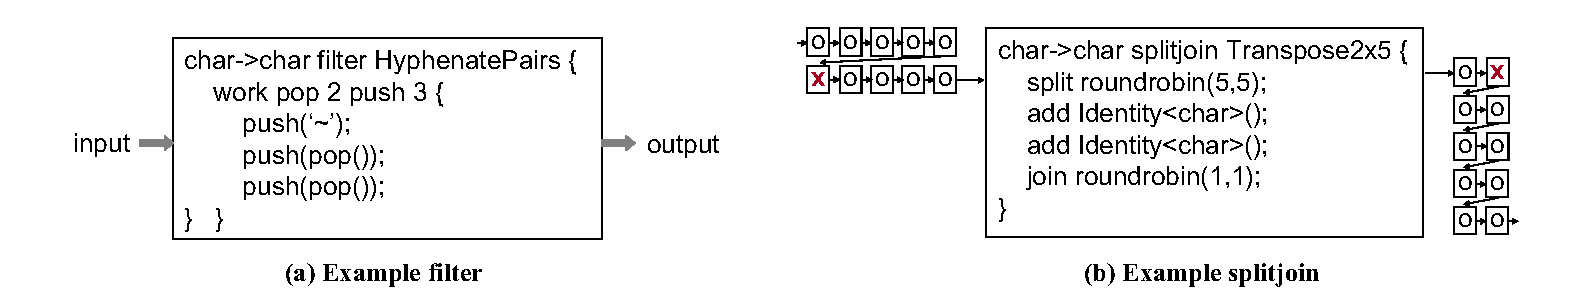
\psfig{file=compressed-filters-in-streamit.eps,width=\textwidth}
\vspace{6pt}
\caption{Example filter, splitter, and joiner in StreamIt.  The
  splitter and joiner combine to form a Transpose. Translation to the
  compressed domain is illustrated in Figures~\ref{fig:filter-example}
  and~\ref{fig:sj-example}.\protect\label{fig:streamit-example}}
\end{figure*}

\begin{figure*}[t]
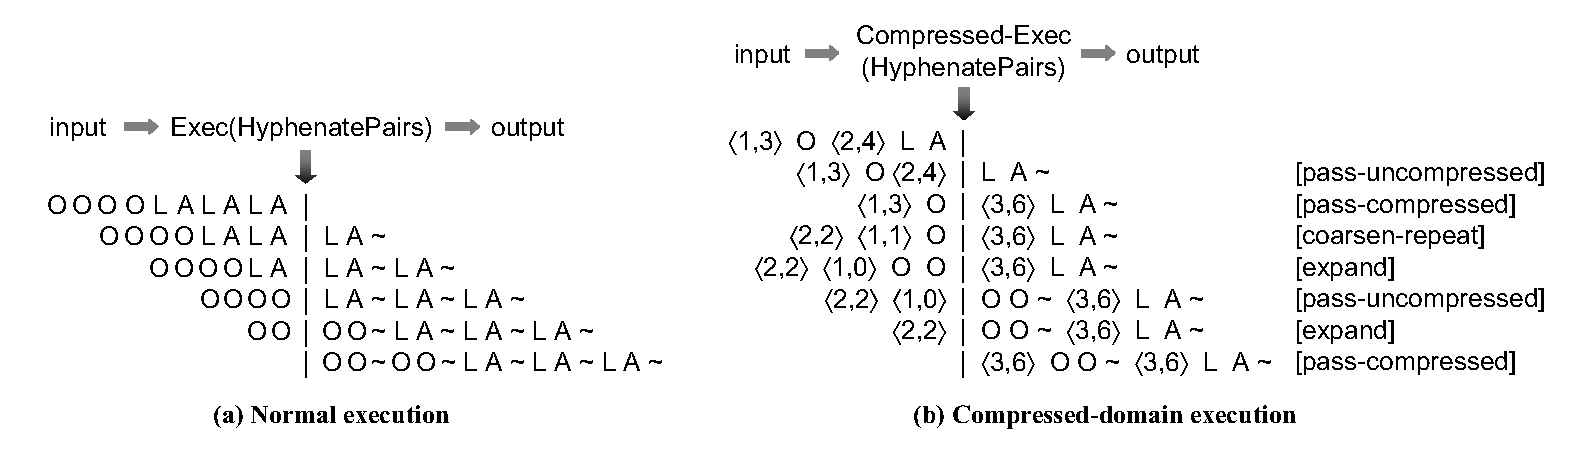
\psfig{file=compressed-filter-example.eps,width=\textwidth}
\vspace{6pt}
\caption{Example execution of a filter in the uncompressed and
  compressed domains.  See Figure~\ref{fig:streamit-example}(a) for the
  source filter.\protect\label{fig:filter-example}}
\end{figure*}

\subsection{Joiners}

%% It is necessary to consider splitters and joiners separately from
%% general-purpose actors because of their pass-through semantics: the
%% inputs are distributed to the outputs without performing any
%% computation.  Our translation to the compressed domain leverages this
%% fact to preserve considerably more compression than would be possible
%% if splitters and joiners were viewed as opaque computational nodes
%% with multiple inputs and multiple outputs.

The procedure for executing a joiner in the compressed domain appears
in Figure~\ref{fig:translate}(b), while an example appears in
Figure~\ref{fig:sj-example}.  To simplify the presentation, we
consider a joiner with only two input streams.  This captures all of
the fundamental ideas; extension to additional streams is
straightforward.  In addition, we use the following notations:

\begin{figure*}[t]
\vspace{-1\baselineskip}
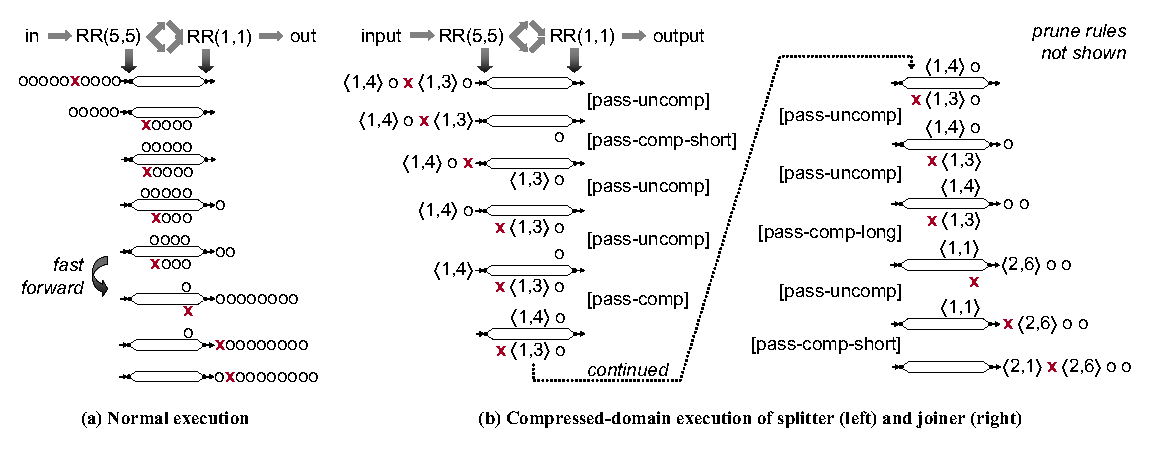
\psfig{file=compressed-splitjoin-example.eps,width=\textwidth}
\caption{Example execution of splitters and joiners in the compressed
  domain.  As illustrated by the input/output pairs in
  Figure~\ref{fig:streamit-example}(b), the example performs a transpose
  of a 2x5 matrix.  When the matrix is linearized as shown here, the
  input stream traverses the elements row-wise while the output stream
  traverses column-wise.  Due to redundancy in the matrix, this
  reordering can be done largely in the compressed domain.
  \protect\label{fig:sj-example}}
\end{figure*}

\begin{itemize}

\vspace{4pt} \item As mentioned previously, splitters and joiners
  adopt a fine-grained cyclo-static execution model, in which each
  execution step transfers only one item from an input tape to an
  output tape.  That is, a roundrobin$(n_1, n_2)$ joiner has $n_1 +
  n_2$ distinct execution steps.  We refer to every group of $n_1 +
  n_2$ steps as an {\it execution cycle}.

\vspace{4pt} \item The pseudocode in Figure~\ref{fig:translate}
  assumes, without loss of generality, that the next execution step of
  the joiner will read from the first input stream (input1).

\vspace{4pt} \item We use $\pos$ to denote the number of items (in
  terms of the uncompressed domain) that have already been read from
  the current input stream (input1) in the current execution cycle.
  For brevity, the pseudocode does not maintain the value of $\pos$,
  though it is straightforward to do so.

\end{itemize}

\begin{figure}[t]
\begin{minipage}{0.1in}
\vspace{-1.75pt}
{\it // // // // // //}
\end{minipage}
\begin{minipage}{3.23in}
{\it Given that $c_1$ and $c_2$ compressed items are available on the
  first and second input streams of a joiner, returns the number of
  items that can be read from each input before one of them is
  exhausted.  Assumes that the joiner is currently reading from the
  first input stream, from which \mbox{pos} items have previously been
  consumed in the current execution cycle.}
\end{minipage}
\textsc{Repeat\_Lengths}$(c_1, c_2, \pos )$~returns~(int,~int)~\{\\
\tab{\it // the number of complete joiner cycles, and the leftovers}\\
\tab$\mbox{total\_cycles} = \mbox{floor}(c/(n_1 + n_2))$\\
\tab$\mbox{leftover}_1 = c_1 - \mbox{total\_cycles} * n_1$\\
\tab$\mbox{leftover}_2 = c_2 - \mbox{total\_cycles} * n_2$\\
~ \vspace{-6pt}\\
\tab{\it // the last partial cycle may end in three regions:}\\
\tab$\mbox{\bf if~} \mbox{leftover}_1 \leq n_1 - \pos$~\{\\
\tab\tab{\it // 1. in reading from the first input stream}\\
\tab\tab$L_1 = \mbox{leftover}_1$\\
\tab\tab$L_2 = 0$\\
\tab$\} \mbox{\bf~else if~} \mbox{leftover}_2 \leq n_2~\{$\\
\tab\tab{\it // 2. in subsequent reading from the second input stream}\\
\tab\tab$L_1 = n_1-\pos$\\
\tab\tab$L_2 = \mbox{leftover}_2$\\
\tab\} \mbox{\bf ~else} \{\\
\tab\tab{\it // 3. in wrap-around reading from the first input stream}\\
\tab\tab$L_1 = \mbox{leftover}_1$\\
\tab\tab$L_2 = n_2$\\
\tab\}\\
~ \vspace{-6pt}\\ 
\tab$\mbox{\bf return~}(n_1*\mbox{total\_cycles} + L_1, n_2*\mbox{total\_cycles} + L_2)$
\}
\caption{The \textsc{Repeat\_Lengths} function is called during
  compressed joiner execution.  In the case where the input tokens to
  the joiner have compatible repeat distances, it calculates the
  maximum repeat lengths that can be passed to the
  output.\protect\label{fig:repeat-lengths}}
\vspace{-2pt}
\end{figure}

There are two ways to pass repeat tokens through a joiner.  If the
input streams contain compatible repeat tokens, then they can be
combined into a long repeat that spans multiple execution cycles;
otherwise, a shorter repeat is extracted from only one of the streams.

The first and most powerful way to execute joiners in the compressed
domain is to combine repeat tokens from both input streams (case {\it
  pass-compressed-long} in Figure~\ref{fig:translate}b).  For this to
be possible, both repeat distances must be the same multiple of their
respective joiner weight ($n_1$ or $n_2$); the combined token has a
repeat distance that is a multiple of $n_1 + n_2$.  The
\textsc{Repeat\_Lengths} routine (detailed in
Figure~\ref{fig:repeat-lengths}) calculates the maximum repeat length
depending on the current position of the joiner and the repeat lengths
of the inputs.

The second mode of compressed joiner execution ({\it
  pass-compressed-short}) inputs only a single repeat token,
extracting the maximum length that can safely move to the output.  The
\textsc{Join\_Potential} routine (detailed in
Figure~\ref{fig:join-potential}) determines how much of the repeat can
be moved to the output before the data referenced would have
originated from a different input stream.
